%==============================================
\subsection{Physics-Informed Hybrid Search}\label{subsec:simloop}

As shown in Fig.~\ref{fig:PIHS}, the physics-informed hybrid search~(PIHS)
couples WCCG-guided gap sequencing, recursive push-task generation,
contact-mode optimization, and short-horizon physics rollout. A search node is a
simulated system snapshot, and a push task labels each tree edge. Auxiliary
records, including parent pointer, incoming task, gap-sequencing cache,
accumulated push effect, and accumulated execution cost, are used only for queue
ordering and solution reconstruction. Thus, WCCG proposes clearance
opportunities, while all state transitions are generated and validated by
physics simulation.

\subsubsection{Tree Initialization and Node Value}
The search tree~$\mathcal{T}$ contains snapshot nodes indexed by~$\nu$, each
associated with a full system state~$\mathbf{s}_\nu$ in~\eqref{eq:transition}.
For a non-root node, let~$\nu^-$ be its parent and~$\tau_\nu$ be the incoming
push task that generates~$\mathbf{s}_\nu$ from~$\mathbf{s}_{\nu^-}$ through
\eqref{eq:sim}. The accepted task sequence is recovered by tracing incoming edge
labels from a terminal node back to the root.

For the simulated edge~$\nu^-\xrightarrow{\tau_\nu}\nu$, the push-effect score is
\begin{equation}\label{eq:push_effect}
\begin{aligned}
\mathsf{E}(\nu)
&\triangleq
\min\{\mathsf{E}_{\max},
\mathsf{E}(\nu^-)+\Delta\mathsf{E}(\nu^-,\nu)\},\\
\Delta\mathsf{E}(\nu^-,\nu)
&\triangleq
\Delta\mathsf{E}_{\mathrm{obs}}(\mathbf{s}_{\nu^-},\mathbf{s}_{\nu})\\
&\quad +b_g\mathbb{I}\{d_g^-\le W+\epsilon<d_g\}
+\gamma_g(d_g-d_g^-),
\end{aligned}
\end{equation}
where~$\mathsf{E}_{\max}$ is a finite cap, or~$\infty$ when clipping is not
used. The term~$\Delta\mathsf{E}_{\mathrm{obs}}$ measures the weighted object-pose
change between parent and child snapshots. The quantities~$d_g^-$ and~$d_g$ are
the selected gap widths before and after rollout, and~$b_g,\gamma_g\ge0$ reward
first opening the gap beyond~$W+\epsilon$ and further enlarging it. Endpoint
clearance omits the gap-width terms. This score is only a search heuristic;
physical validity is decided by~\eqref{eq:sim}.

The accumulated execution cost is
\begin{equation}\label{eq:exec_cost}
\begin{aligned}
\mathsf{C}(\nu)
&\triangleq
\mathsf{C}(\nu^-)+\Delta\mathsf{C}(\nu^-,\nu),\\
\Delta\mathsf{C}(\nu^-,\nu)
&\triangleq
T_{\mathrm{roll}}(\nu^-,\nu)
+\lambda_{\mathrm{tr}}\widehat{C}_{\mathrm{tr}}(\tau_\nu;\mathbf{s}_{\nu^-}),
\end{aligned}
\end{equation}
where~$T_{\mathrm{roll}}$ is rollout duration or control-step count, and
$\widehat{C}_{\mathrm{tr}}$ estimates robot-transfer cost for reaching the
contact configuration of~$\tau_\nu$. The open queue uses
\begin{equation}\label{eq:node_value}
f(\nu)\triangleq
\overline{\mathsf{J}}_{\mathrm{clr}}(\mathbf{s}_\nu)
+(1-\beta)\overline{\mathsf{C}}(\nu)
-\beta\overline{\mathsf{E}}(\nu),
\end{equation}
where~$\overline{\mathsf{J}}_{\mathrm{clr}}$ is the normalized W--clearance
cost-to-go from~\eqref{eq:state_c2g}, and~$\overline{\mathsf{C}}$ and
$\overline{\mathsf{E}}$ are normalized branch cost and push-effect scores. The
parameter~$\beta\in[0,1]$ trades optimality for aggressive feasibility search in
dense scenes. Duplicate quantized snapshots are filtered by keeping the
shallowest occurrence.

\subsubsection{Expansion by Lazy Recursive Task Batches}
At each iteration, the node with minimum~\eqref{eq:node_value} is popped and gap
sequencing is run on~$\mathbf{s}_\nu$. If~\eqref{eq:wccg_criterion} already
succeeds, the task sequence traced from the root is returned. If an endpoint is
blocked, endpoint-clearance tasks are sampled by treating the endpoint as a
virtual obstacle. Otherwise, the first portal gap of the best gap sequence is
selected. The sampler first emits direct pushing tasks. If these rollouts break
the target gap, improve the WCCG clearance estimate, or exceed the lazy-progress
threshold, recursive expansion is skipped. Recursive blocker-clearing tasks are
released only when the direct batch makes insufficient progress, or immediately
when the same gap is revisited under eager direct-plus-recursive sampling. Each
accepted rollout creates a child snapshot, sorted by~\eqref{eq:node_value},
limited by the child budget, and inserted into a capped open queue.

%==============================================
\begin{algorithm}[t!]
\caption{Physics-Informed Hybrid Search}\label{alg:push}
\SetAlgoLined
\KwIn{$\mathbf{s}_0$, clearance~$W$, child budget~$B$, greediness~$\beta$,
simulator~$\mathsf{EvalSim}$}
\KwOut{push-task sequence~$\pi^\star$}
create root node~$\nu_0$ with~$\mathbf{s}_{\nu_0}\gets\mathbf{s}_0$,
$\mathsf{E}(\nu_0)\gets0$, $\mathsf{C}(\nu_0)\gets0$,
$\mathcal{Q}\gets\{\nu_0\}$\;
\While{$\mathcal{Q}\neq\emptyset$}{
  $\nu\gets\mathcal{Q}.\texttt{pop\_min}()$ by~\eqref{eq:node_value}\;
  $\mathcal{R}_{\nu}\gets\texttt{GapSequencing}(\mathbf{s}_{\nu})$\;
  \If{$\mathbf{s}_{\nu}$ satisfies~\eqref{eq:wccg_criterion}}{
    \Return~$\texttt{TraceTasks}(\nu)$\;
  }
  \eIf{an endpoint is blocked in $\mathcal{R}_{\nu}$}{
    $\mathcal{B}\gets\texttt{SampleEndpointTasks}(\mathbf{s}_{\nu},B)$\;
    $\mathcal{C}\gets\texttt{EvalBatch}(\mathcal{B},\mathbf{s}_{\nu})$\;
  }{
    $g^\star\gets\texttt{FirstGap}(\mathcal{R}_{\nu})$\;
    $\mathcal{B}_{\mathrm{d}}\gets\texttt{SampleDirectTasks}(g^\star,B)$\;
    $\mathcal{C}\gets\texttt{EvalBatch}(\mathcal{B}_{\mathrm{d}},\mathbf{s}_{\nu})$\;
    \If{$\mathcal{C}$ yields no lazy progress}{
      $\mathcal{B}_{\mathrm{r}}\gets\texttt{SampleRecursiveTasks}(g^\star,B)$\;
      $\mathcal{C}\gets\mathcal{C}\cup
      \texttt{EvalBatch}(\mathcal{B}_{\mathrm{r}},\mathbf{s}_{\nu})$\;
    }
  }
  \ForEach{$(\tau,\mathbf{s}',\rho)\in\mathcal{C}$}{
    create child node~$\nu'$ with~$\mathbf{s}_{\nu'}\gets\mathbf{s}'$,
    parent~$\nu$, and incoming task~$\tau$\;
    update~$\mathsf{E}(\nu')$, $\mathsf{C}(\nu')$, and~$f(\nu')$\;
    $\mathcal{Q}.\texttt{push}(\nu')$\;
  }
  trim duplicate snapshots and cap~$\mathcal{Q}$\;
}
\Return~failure\;
\end{algorithm}
%==============================================

%==============================
\begin{figure*}[t!]
  \centering
  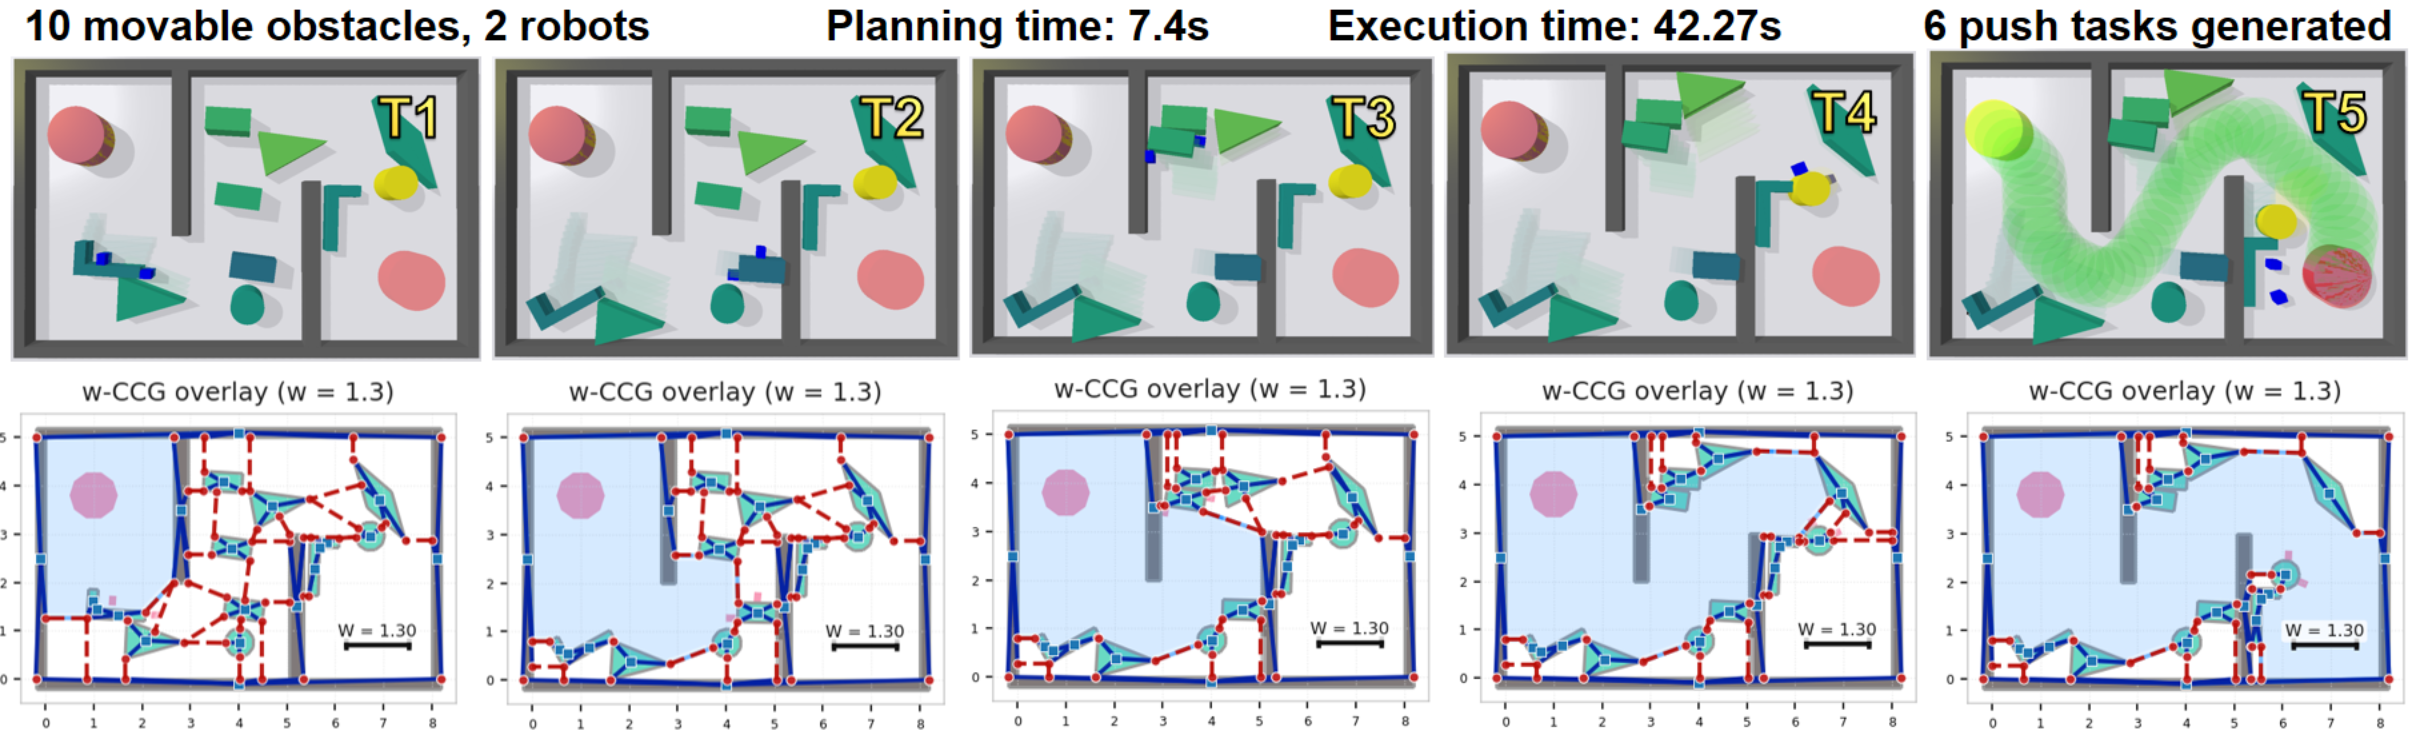
\includegraphics[width=0.95\linewidth]{figures/sim_exp.png}
  \vspace{-0.15in}
\caption{Execution--planning alignment in the main scenario.
\textbf{Top:}~$5$ PyBullet snapshots as~$2$ robots push a cylindrical object.
\textbf{Bottom:} corresponding WCCG overlays with the start face in blue.
The task moves the object from
\(\mathbf{s}^{\texttt{S}}_{\texttt{V}}=(1,4)\) to
\(\mathbf{s}^{\texttt{G}}_{\texttt{V}}=(7,2)\).
In the final state, the start face contains~$G$, matching the executed
trajectory and confirming success.}
\vspace{-0.1in}
\label{fig:simloop}
\end{figure*}
% ========================================

\subsubsection{Termination and Replanning}
Termination occurs when a popped node~$\nu$ reaches a snapshot satisfying the
WCCG clearance certificate in~\eqref{eq:wccg_criterion}. The solution
$\pi^\star$ is obtained by tracing incoming push-task labels to the root and
constitutes a complete solution to~\eqref{eq:problem}. During execution, WCCG,
gap-sequencing cache, and reusable ModeTable entries are updated after each
accepted task. If object drift, transition blockage, or contact loss invalidates
the remaining prefix, the search restarts from the observed snapshot while
preserving failed task signatures and reusable mode entries.
